%-----------------------------------------------------------------------------%
\chapter{\babDua}
%-----------------------------------------------------------------------------%
%-----------------------------------------------------------------------------%
Bab ini membahas tentang konsep dan teori yang mendasari penelitian Tugas Akhir ini yang meliputi tentang DVB-T2, LDPC \textit{codes}, standar LDPC \textit{codes} DVB-T2, algoritma \textit{Progressive Edge-Growth} (PEG) untuk LDPC \textit{codes}, modulasi QPSK, \textit{Orthogonal Frequency Division Multiplexing} (OFDM), pemodelan kanal yang digunakan, dan EXIT \textit{chart}.


%-----------------------------------------------------------------------------%
\section{\textit{Digital Video Broadcasting – Second Generation Terrestrial} (DVB-T2)}
%-----------------------------------------------------------------------------%
DVB-T2 merupakan standar untuk penyiaran televisi digital yang telah ditetapkan oleh ETSI. DVB-T2 memiliki kinerja lebih baik daripada generasi sebelumnya yaitu DVB-T. DVB-T2 memiliki banyak perbedaan dengan DVB-T salah satunya adalah FEC DVB-T2 yang menggunakan Bose Chaudhuri Hocquenghem (BCH) \textit{codes} dan LDPC \textit{codes}. Dampak penggunaan FEC ini, memberikan keunggulan pada DVB-T2, sehingga memiliki laju data yang lebih cepat $30\%$ daripada DVB-T dan memungkinkan DVB-T2 untuk menggunakan 256-QAM, \textit{Fast Fourier Transform} (FFT) \textit{size} sebesar 16K dan 32K, serta diagram konstelasi yang berotasi. \text{Akibatnya}, memungkinkan untuk mengirimkan kualitas video \textit{High Definition Television Video} (HDTV) \cite{etsi2}.

\begin{table} [tb]
	\renewcommand{\figurename}{Table}
	\centering 
	\caption{Distribusi \textit{column weight} LDPC \textit{codes} DVB-T2 \textit{short frame}.}
	\label{table:dvb-t2lite}
	\begin{tabular}{|c|c|c|c|c|c|c|c|}
		\hline
		\multicolumn{2}{|c|}{Code rate} & \multicolumn{6}{c|}{Column weight}    \\ \hline
		$R_n$  & $R_e$  & 13   & 12   & 8    & 3     & 2    & 1 \\ \hline
		1/2           & 4/9             &      &      & 1800 & 5400  & 8999 & 1 \\ \hline
		3/5           & 3/5             &      & 3240 &      & 6480  & 6479 & 1 \\ \hline
		2/3           & 2/3             & 1080 &      &      & 9720  & 5399 & 1 \\ \hline
		3/4           & 11/15           &      & 360  &      & 11520 & 4319 & 1 \\ \hline
		4/5           & 7/9             &      &      &      & 12600 & 3599 & 1 \\ \hline
		5/6           & 37/45           & 360  &      &      & 12960 & 2879 & 1 \\ \hline
	\end{tabular}
	
	
\end{table}

LDPC \textit{codes} merupakan \textit{inner coding} dari FEC DVB-T2, \textit{code rate} dari LDPC \textit{codes} yang telah ditentukan oleh standar dari ETSI, yaitu : $\frac{1}{2}, \frac{3}{5}, \frac{2}{3}, \frac{3}{4}, \frac{4}{5},$ atau $\frac{5}{6}$ \cite{etsi2}. \textit{Code rate} sebesar $\frac{1}{2}$ memiliki perlindungan proteksi maksimal dan laju data minimal, sedangkan untuk \textit{code rate} sebesar $\frac{5}{6}$ memiliki perlindungan proteksi minimal dan laju data maksimal. Sesuai standar ETSI, LDPC \textit{codes} dari DVB-T2 menggunakan struktur \textit{cyclic} di bagian informasi dan struktur \textit{staircase} di bagian \textit{parity}. Untuk panjang blok di LDPC \textit{codes} dapat menggunakan 16.200 blok (\textit{short frame}) yang akan lebih baik untuk laju data rendah dan 64.800 blok (\textit{long frame}) yang akan lebih baik untuk laju data yang lebih tinggi. Pembentukan matriks \textit{parity check} LDPC \textit{codes} DVB-T2 dibuat berdasarkan dari Tabel \textit{Addresses Parity Bit Accumulator}-nya. Kinerja dari LDPC \textit{codes} akan dipengaruhi oleh \textit{code rate}, lebar spektrum frekuensi, \textit{Guard Interval} (GI), panjang \textit{frame}, dan parameter transmisi lainnya.

\begin{table}[tb]
\centering
\caption{\textit{Addresses of parity bit accumulators} untuk $N_{LDPC}=16200$ dengan \textit{code rate} $R_e=\frac{4}{9}$.}
\label{table:adressldpc}
		\begin{tabular}{|l|l|l|lllll}
			\hline
			\multicolumn{1}{|c|}{20} & \multicolumn{1}{c|}{712}  & \multicolumn{1}{c|}{2386} & \multicolumn{1}{c|}{6354} & \multicolumn{1}{c|}{4061} & \multicolumn{1}{c|}{1062} & \multicolumn{1}{c|}{5045} & \multicolumn{1}{c|}{5158} \\ \hline
			\multicolumn{1}{|c|}{21} & \multicolumn{1}{c|}{2543} & \multicolumn{1}{c|}{5748} & \multicolumn{1}{c|}{4822} & \multicolumn{1}{c|}{2348} & \multicolumn{1}{c|}{3089} & \multicolumn{1}{c|}{6328} & \multicolumn{1}{c|}{5876} \\ \hline
			\multicolumn{1}{|c|}{22} & \multicolumn{1}{c|}{926}  & \multicolumn{1}{c|}{5701} & \multicolumn{1}{c|}{269}  & \multicolumn{1}{c|}{3693} & \multicolumn{1}{c|}{2438} & \multicolumn{1}{c|}{3190} & \multicolumn{1}{c|}{3507} \\ \hline
			\multicolumn{1}{|c|}{23} & \multicolumn{1}{c|}{2802} & \multicolumn{1}{c|}{4520} & \multicolumn{1}{c|}{3577} & \multicolumn{1}{c|}{5324} & \multicolumn{1}{c|}{1091} & \multicolumn{1}{c|}{4667} & \multicolumn{1}{c|}{4449} \\ \hline
			\multicolumn{1}{|c|}{24} & \multicolumn{1}{c|}{5140} & \multicolumn{1}{c|}{2003} & \multicolumn{1}{c|}{1263} & \multicolumn{1}{c|}{4742} & \multicolumn{1}{c|}{6497} & \multicolumn{1}{c|}{1185} & \multicolumn{1}{c|}{6202} \\ \hline
			0                        & 4046                      & 6934                      &                           &                           &                           &                           &                           \\ \cline{1-3}
			1                        & 2855                      & 66                        &                           &                           &                           &                           &                           \\ \cline{1-3}
			2                        & 6694                      & 212                       &                           &                           &                           &                           &                           \\ \cline{1-3}
			3                        & 3439                      & 1158                      &                           &                           &                           &                           &                           \\ \cline{1-3}
			4                        & 3850                      & 4422                      &                           &                           &                           &                           &                           \\ \cline{1-3}
			5                        & 5924                      & 290                       &                           &                           &                           &                           &                           \\ \cline{1-3}
			6                        & 1467                      & 4049                      &                           &                           &                           &                           &                           \\ \cline{1-3}
			7                        & 7820                      & 2242                      &                           &                           &                           &                           &                           \\ \cline{1-3}
			8                        & 4606                      & 3080                      &                           &                           &                           &                           &                           \\ \cline{1-3}
			9                        & 4633                      & 7877                      &                           &                           &                           &                           &                           \\ \cline{1-3}
			10                       & 3884                      & 6868                      &                           &                           &                           &                           &                           \\ \cline{1-3}
			11                       & 8935                      & 4996                      &                           &                           &                           &                           &                           \\ \cline{1-3}
			12                       & 3028                      & 764                       &                           &                           &                           &                           &                           \\ \cline{1-3}
			13                       & 5988                      & 1057                      &                           &                           &                           &                           &                           \\ \cline{1-3}
			14                       & 7411                      & 3450                      &                           &                           &                           &                           &                           \\ \cline{1-3}
		\end{tabular}

	
\end{table}

%-----------------------------------------------------------------------------%
\section{\textit{Low Density Parity Check} (LDPC) \textit{Codes}}
%-----------------------------------------------------------------------------%
LDPC \textit{codes} atau dapat disebut juga \textit{Gallager's codes} diusulkan pada tahun 1962 oleh Robert Gallager \cite{ldpc1}. LDPC \textit{codes} merupakan sebuah \textit{channel coding} untuk melakukan \textit{error correction} yang menggunakan pengkodean dengan menggunakan matriks generator berukuran besar yang jumlah elemen 1 lebih sedikit dibandingkan elemen 0, sehingga disebut \textit{low-density codes} \cite{QC1}. Elemen 1 menunjukkan hubungan antara bit masukan \text{dengan} bit keluaran dari LDPC \textit{codes}. MacKay merupakan salah satu peniliti yang telah menunjukkan bahwa LDPC \textit{codes} memiliki kinerja yang mendekati kapasitas Shannon \cite{ldpc3,ldpc4,ldpc5}. 
%LDPC \textit{codes} mampu meningkatkan reliabilitas dengan menambahkan bit \textit{parity} yang dikirimkan bersamaan dengan bit informasi. Reliabilitas LDPC \textit{codes} semakin lebih baik karena sifat \textit{low-density} pada matriks \textit{parity check}-nya, 

Generator matriks LDPC \textit{codes} ($\mathbf{G}$) berfungsi sebagai pembentuk \textit{codeword} dari bit informasi di sisi pengirim dan matriks \textit{parity check} ($\mathbf{H}$) untuk mengembalikan \textit{codeword} menjadi bit informasi. Keduanya harus memenuhi 
\begin{equation}
\mathbf{G} \mathbf{H}^{T} = 0.
\label{eq:GH}
\end{equation}
Jika Persamaan (\ref{eq:GH}) tidak terpenuhi, LDPC \textit{codes} tidak dapat mendeteksi dan mengoreksi \textit{error} atas \textit{codeword} yang diterima. Bentuk matriks \textit{parity check} dari LDPC \textit{codes} disesuaikan dengan panjang blok (N), dimensi (K), redudansi (M), \textit{degree of variable node} ($d_{v}$), dan \textit{degree of check node} ($d_{c}$) dengan 
\begin{equation}
M = N-K,
\label{eq:Redudansi LDPC code}
\end{equation}
maka matriks \textit{parity check} LDPC \textit{codes} memiliki dimensi $M \times N$. \textit{Variable node} digunakan untuk mendeskripsikan setiap kolom dan \textit{check node} untuk setiap baris dari matriks LDPC \textit{codes}. 
%LDPC \textit{codes} terbagi menjadi dua, yaitu: \textit{regular} yang memiliki nilai $d_{v}$ dan $d_{c}$ sama di setiap baris maupun kolom  dan \textit{irregular} memiliki nilai $d_{v}$ dan $d_{c}$ yang berbeda di baris dan kolom yang memiliki kinerja mengungguli \textit{regular} LDPC \textit{codes} \cite{ldpc7}. 

\begin{figure}
	\centering
	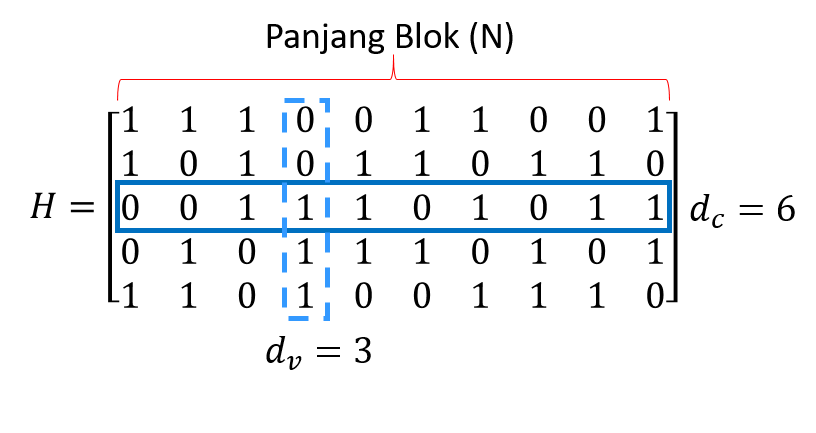
\includegraphics[width=0.6\textwidth]
		{pics/diagram/ldpc.png}
		\caption{Matriks \textit{parity check} \textit{regular} LDPC \textit{codes} (3,6).}
	\label{fig:Regular LDPC codes (3,6)}
\end{figure}
\begin{figure}
	\centering
	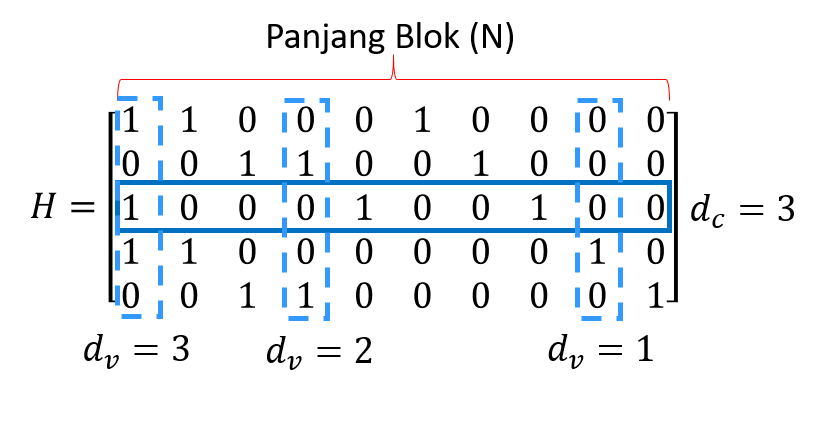
\includegraphics[width=0.6\textwidth]
		{pics/diagram/irre.png}
		\caption{Matriks \textit{parity check} \textit{irregular} LDPC \textit{codes}.}
	\label{fig:Irregular LDPC codes}
\end{figure}
%\textit{Irregular} LDPC \textit{codes} memiliki beban kolom dan beban baris yang berbeda-beda, secara substansial mengungguli \textit{regular} LDPC \textit{codes} \cite{ldpc7}. \textit{Irregular} LDPC \textit{codes} memiliki rumus distribusi kolom $\lambda (x)$ dan distribusi baris $\rho (x)$, sebagai berikut:
%\begin{equation}
%\lambda (x)=\sum_{i= 2}^{dv}\lambda_{i}x^{i-1}
%\label{eq:Distribusi Kolom Kode LDPC Irregular}
%\end{equation}
%\begin{equation}
%\rho (x)=\sum_{i= 2}^{dc}\rho_{i}x^{i-1}
%\label{eq:Distribusi Baris Kode LDPC Irregular}
%\end{equation}
%Dengan asumsi semua persamaan $\lambda (x)$ dan $\rho (x)$ bersifat saling independen secara linier, maka R atau \textit{rate} dari \textit{Irregular} LDPC \textit{codes} adalah 
%\begin{equation}
%R(\lambda,\rho) = 1-\frac{\int_{0}^{1}\rho (x)dx}{\int_{0}^{1}\lambda (x)dx}
%\label{eq:Kode LDPC Irregular}
%\end{equation}
\subsection{Tanner\textit{ Graph}}
Tanner\textit{ graph} merupakan \textit{bipartite graph} yang digunakan untuk menyatakan batasan atau persamaan dari sebuah \textit{error corecting codes} \cite{tann1}. Matriks \textit{parity check} LDPC \textit{codes} dapat direpresentasikan dalam bentuk graf yaitu Tanner\textit{ graph} yang terdiri dari beberapa set \textit{node}. Tanner\textit{ graph} memiliki sebuah garis yang menghubungkan antara \textit{variable node} dan \textit{check node}, jika dan hanya jika \textit{variable node} memiliki hubungan dengan \textit{check node}. Gambar \ref{fig:Tanner Graph LDPC Regular (3,6)} menunjukkan Tanner\textit{ graph} dari matriks \textit{parity check} pada Gambar \ref{fig:Regular LDPC codes (3,6)}, sedangkan Gambar \ref{fig:tg Irregular LDPC codes} merupakan bentuk Tanner\textit{ graph irregular} LDPC \textit{codes} yang memiliki distribusi \textit{variable node degree} (VND) $\Lambda (x)$ dan \textit{check node degree} (CND) $\Omega (x)$ sebagai berikut:
\begin{equation}
 \Lambda (x)=\frac{3}{12}x^{2}+\frac{7}{12}x^{3}+\frac{1}{12}x^{4}+\frac{1}{12}x^{5},
\label{eq:Distribusi var nodes rregular LDPC codes}
\end{equation}
\begin{equation}
 \Omega (x)=\frac{1}{6}x^{4}+\frac{2}{6}x^{5}+\frac{1}{6}x^{6}+\frac{2}{6}x^{7}.
\label{eq:Distribusi check nodes rregular LDPC codes}
\end{equation}
% serta untuk gambar \ref{fig:tg Irregular LDPC codes} Irregular LDPC codes} mewakili \textit{Tanner Graph} dari gambar \ref{fig:Irregular LDPC codes}.
\begin{figure}[tb]
	\centering
	\includegraphics[width=0.35\textwidth]
		{pics/diagram/ldpc2.png}
		\caption{Tanner\textit{ graph} matriks \textit{parity check} \textit{regular} LPDC \textit{codes} dengan $d_{v}=3$ dan $d_{c}=6$.}
	\label{fig:Tanner Graph LDPC Regular (3,6)}
\end{figure} 
\begin{figure}
	\centering
	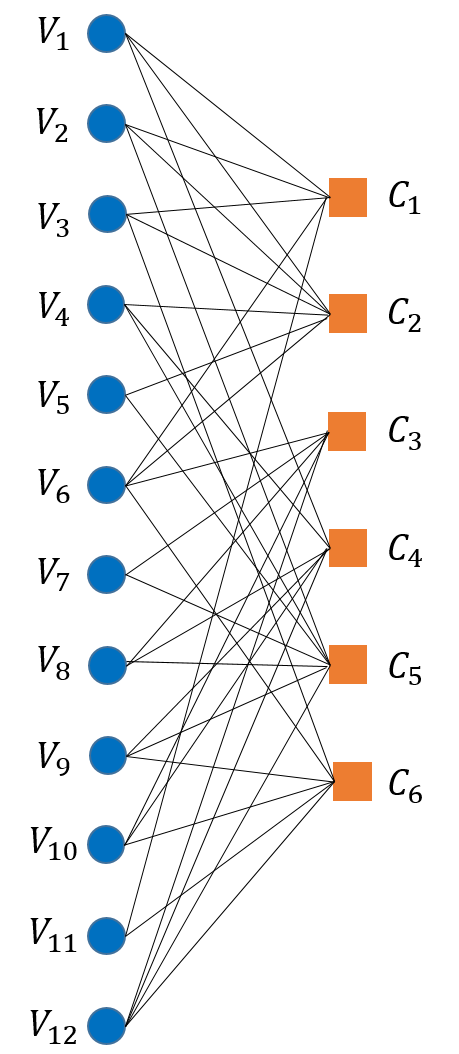
\includegraphics[width=0.32\textwidth]
		{pics/diagram/ldpc3.png}
		\caption{Tanner\textit{ graph} matriks \textit{parity check} \textit{irregular} LDPC \textit{codes} dengan $\Lambda(x)$ pada (\ref{eq:Distribusi var nodes rregular LDPC codes}) dan $\Omega(x)$ pada (\ref{eq:Distribusi check nodes rregular LDPC codes}).}
	\label{fig:tg Irregular LDPC codes}
\end{figure} 

\subsection{\textit{Girth}}
\begin{figure}[b]
	\centering 
	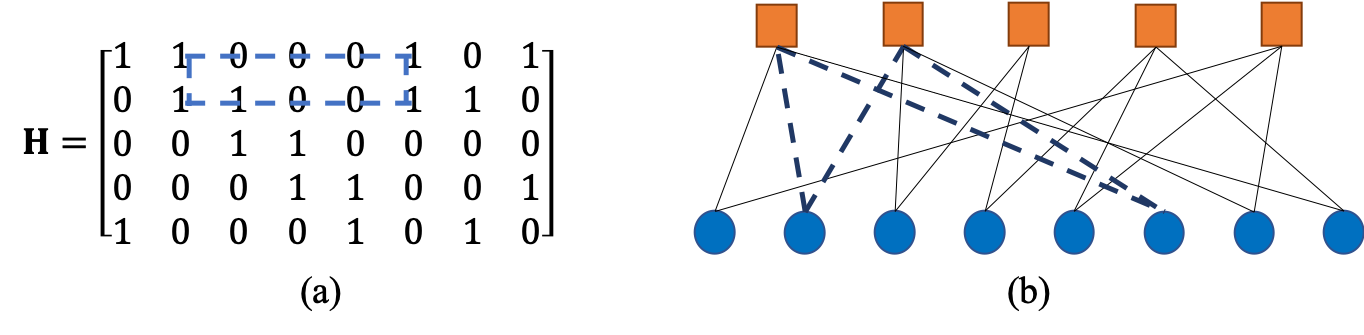
\includegraphics[scale=0.6]{pics/GirthH2}
	\centering 
	\caption{Sebuah contoh \textit{girth} 4 pada LDPC \textit{codes} dengan \textit{cycle} ditunjukkan dengan garis putus-putus: (a) dalam matriks \textit{parity check} $\mathbf{H}$ dan (b) dalam Tanner \textit{graph}.}
	\label{fig:girth}
\end{figure}

	 \textit{Girth} adalah panjang siklus terpendek dalam sebuah Tanner \textit{graph} yang menjadi hal penting dalam menentukan kinerja LDPC \textit{codes} \cite{girth}. Adapun \textit{girth} lokal, \textit{girth} lokal ini terbentuk dari siklus per-\textit{node} pada sebuah Tanner \textit{graph} LDPC \textit{codes}. \textit{Girth} terkecil yang mungkin muncul pada LDPC \textit{codes} adalah \textit{girth} 4, oleh karena itu pada perancangan LDPC \textit{codes} munculnya \textit{girth} 4 harus dihindari. \textit{Girth} dapat dihitung dengan mudah dengan mengamati Tanner \textit{graph} yang terbentuk pada LDPC \textit{codes}. Untuk \textit{girth} 4 dapat diamati melalui matriks \textit{parity check} LDPC \textit{codes} dengan mengamati elemen 1 yang ada, apabila terdapat elemen 1 yang membentuk persegi atau persegi panjang maka \textit{girth} 4 pasti muncul pada LDPC \textit{codes} tersebut seperti pada Gambar \ref{fig:girth}. \textit{Girth} kecil pada LDPC \textit{codes} akan memberikan efek buruk pada LDPC \textit{codes}, karena mengurangi kinerja dari \textit{extrinsic information} dalam proses \textit{iterative decoding} LDPC \textit{codes} \cite{girth2}.

\subsection{\textit{Regular} LDPC \textit{Codes}}
\textit{Regular} LDPC \textit{codes} merupakan struktur LDPC \textit{codes} yang memiliki nilai $d_{v}$ atau banyaknya nilai 1 di setiap kolomnya sama dan nilai $d_{c}$ atau banyaknya nilai 1 di setiap kolomnya sama. Gambar \ref{fig:Regular LDPC codes (3,6)} merupakan contoh matriks dari \textit{regular} LDPC \textit{codes} yang memiliki nilai $N$ sama dengan 10, $d_{v}$ sama dengan 3, dan $d_{c}$ sama dengan 6. Nilai \textit{code rate} \textit{regular} LDPC \textit{codes} dapat diketahui dengan
\begin{equation}
R=1-\frac{d_{v}}{d_{c}}.
\label{code rate regular LDPC codes}
\end{equation}
\subsection{\textit{Irregular} LDPC \textit{Codes}}
\textit{Irregular} LDPC \textit{codes} merupakan jenis struktur dari LDPC \textit{codes} yang memiliki nilai $d_{v}$ dan $d_{c}$ yang tidak sama di setiap baris dan kolomnya, dari segi kinerja \textit{irregular} LDPC \textit{codes} dapat mengungguli \textit{regular} LDPC \textit{codes} \cite{ldpc7}. Hal ini dikarenakan, nilai \textit{girth} dari \textit{irregular} LDPC \textit{codes} cenderung lebih besar dari \textit{regular} LDPC \textit{codes}. \textit{Irregular} LDPC \textit{codes} memiliki persamaan untuk distribusi VND $\Lambda (x)$ dan distribusi CND $\Omega (x)$, sebagai berikut:
\begin{equation}
\Lambda (x)=\sum_{i= 1}^{dv}\Lambda_{i}x^{i},
\label{eq:Distribusi Kolom Irregular LDPC codes}
\end{equation}
\begin{equation}
\Omega (x)=\sum_{i= 1}^{dc}\Omega_{i}x^{i}
\label{eq:Distribusi Baris Irregular LDPC codes}
\end{equation}
dengan asumsi semua persamaan $\Lambda (x)$ dan $\Omega (x)$ bersifat saling independen linier, maka \textit{code rate} $(R)$ dari \textit{irregular} LDPC \textit{codes} adalah 
\begin{equation}
R(\Lambda,\Omega) = 1-\frac{\int_{0}^{1}\Omega (x)dx}{\int_{0}^{1}\Lambda (x)dx}.
\label{eq:Rate Irregular LDPC codes}
\end{equation}

%\subsection{\textit{Quasi-Cyclic} (QC) LDPC \textit{Codes}}
%QC-LDPC \textit{codes} adalah \textit{channel coding} yang memiliki kompleksitas rendah dengan menggunakan struktur dari LDPC \textit{codes} \cite{QC2}. QC-LDPC \textit{codes} memiliki struktur yang terbentuk dari pergeseran sirkular sehingga satu \textit{codeword} yang akan menghasilkan \textit{codeword} lain. Struktur tersebut membuat QC-LDPC \textit{codes} memerlukan memori yang lebih sedikit dibandingkan dengan LDPC \textit{codes} konvensional dan ini merupakan salah satu kelebihan QC-LDPC \textit{codes} \cite{QC3}. Susunan matriks generator dari QC-LDPC \textit{codes} berbeda dengan LDPC \textit{codes} karena QC-LDPC \textit{codes} memiliki matriks yang sirkular. QC-LDPC \textit{codes} memiliki $H_{Q}$ yang terdiri dari beberapa matriks \textit{binary polinomial} yaitu
%\begin{equation}
%H_{Q}(\lambda_{I,J})= \begin{bmatrix} \lambda_{0,0}(U) & \lambda_{0,1}(U) & \cdots & \lambda_{0,J-1}(U) \\ \lambda_{1,0}(U) & \lambda_{1,1}(U) & \cdots & \lambda_{1,J-1}(U) \\ \vdots & \vdots & \ddots & \vdots \\ \lambda_{I-1,0}(U) & \lambda_{I-1,1}(U) & \cdots & \lambda_{I-1,J-1}(U)
%
%\end{bmatrix},
%\label{eq: Matriks Binary Polynomial QC-LDPC}
%\end{equation} 
%
%dengan nilai $I=\{ 0,1,2,\dots,I-1 \}$ adalah jumlah elemen baris dan $J=\{ 0,1,2,\dots,J-1 \}$ adalah elemen kolom matriks $H_{Q}$. Setiap matriks \textit{binary polinomial} $\lambda_{I,J}(U)$ terdiri atas $ZxZ$ matriks \textit{polinomial circular} yaitu
%\begin{equation}
%\lambda_{I,J}(U)= \begin{bmatrix} 
%a_{1} & a_{2} & \cdots & a_{z-1} & a_{z}  \\ 
%a_{z} & a_{1} & \cdots & a_{z-2} & a_{z-1} \\ 
%\vdots & \vdots & \ddots & \vdots & \vdots \\ 
%a_{2} & a_{3} & \cdots & a_{z} & a_{1}
%
%\end{bmatrix}.
%\label{eq: Matriks Binary Polynomial QC-LDPC}
%\end{equation} 
 
\subsection{LDPC \textit{Staircase} \textit{Codes}}
LDPC \textit{Staircase codes} merupakan LDPC \textit{codes} yang menggunakan struktur matriks \textit{lower triangular}. Matriks LDPC \textit{Staircase codes} memiliki bentuk seperti "tangga" yang terbentuk oleh elemen 1, sehingga setiap simbol yang \textit{error} dapat dikoreksi dari nilai jumlah simbol sebelumnya di baris terkait \cite{staircase1}. Matriks \textit{parity check} LDPC \textit{Staircase codes} memiliki bentuk
\begin{equation}
\mathbf{H} = \begin{bmatrix} 
0 & 1 & 1 & 0 & 1 & 0 & \textbf{1} & 0 & 0 & 0  \\ 
1 & 0 & 0 & 1 & 1 & 0 & \textbf{1} & \textbf{1} & 0 & 0  \\ 
0 & 1 & 0 & 1 & 0 & 1 & 0 & \textbf{1} & \textbf{1} & 0  \\ 
1 & 0 & 1 & 0 & 0 & 1 & 1 & 0 & \textbf{1} & \textbf{1} 
\end{bmatrix}.
\label{eq: Matriks Parity Check LDPC-Staircase codes}
\end{equation} 
\noindent Matriks (\ref{eq: Matriks Parity Check LDPC-Staircase codes}) dibagi menjadi dua bagian ($\mathbf{H}_1 \mid \mathbf{H}_2$). $\mathbf{H}_1$ merupakan bagian sebelah kiri matriks $\mathbf{H}$ dari kolom $0$ ke $K-1$ yang mendefinisikan penempatan simbol dari sumber informasi dalam sebuah persamaan linier. $\mathbf{H}_2$ merupakan bagian sebelah kanan matriks $\mathbf{H}$ dari $K$ ke $N-1$ yang mendefinisikan persamaan-persamaan simbol perbaikan pada baris yang berkaitan dan membentuk seperti "tangga". Operasi dasar dalam pembentukan matriks \textit{parity check} LDPC \textit{Staircase codes} menggunakan operasi \textit{exclusive or} (XOR). LDPC \textit{Staircase codes} yang memiliki nilai \textit{code rate} ($R$) setiap $m$ baris dari matriks $\mathbf{H}_1$ akan memiliki \textit{degree}
\begin{equation}
d_{R_{\mathbf{H}_1}}= \frac{N_{1}}{\frac{1}{R}-1}
\label{eq: degree matriks H1}
\end{equation} 
\noindent dengan $N_{1}$ merupakan jumlah banyaknya nilai elemen 1 di setiap kolom matriks $\mathbf{H}_1$ Matriks (\ref{eq: Matriks Parity Check LDPC-Staircase codes}). Akibat dari struktur \textit{staircase} di matriks $\mathbf{H}_2$, satu baris $m$ dari matriks $\mathbf{H}$ akan memiliki \textit{degree}
\begin{equation}
d_{r}(m)=
\left\{\begin{matrix}
d_{r_{\mathbf{H}_1}}+1 \;\;\; if \; m=1,
\\ 
d_{r_{\mathbf{H}_1}}+2 \;\;\; if \; m>1 .
\end{matrix}\right.
\label{eq: degree matriks $H_{1}$}
\end{equation} 
Representasi LDPC \textit{Staircase} \textit{codes} dalam bentuk Tanner\textit{ graph} ditunjukkan oleh Gambar \ref{fig:Tanner Graph LDPC Staircase codes}.

\begin{figure}[t!]
	\centering
	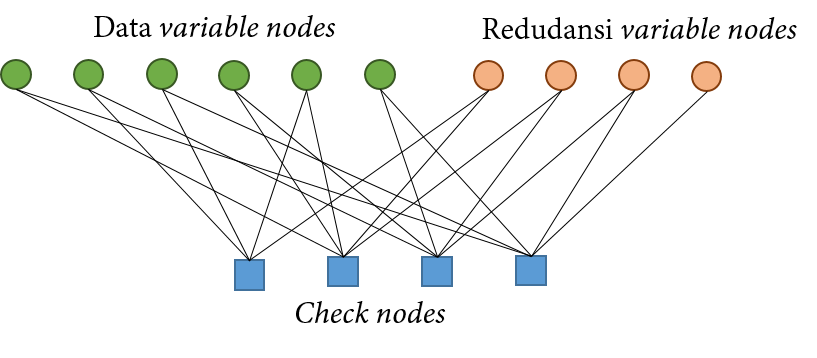
\includegraphics[scale=0.9]
	{pics/staircase.png}
	\caption{\textit{Sebuah Tanner graph} dari LDPC \textit{Staircase codes} dengan $N=10$, $K=6$, dan $N_{1}=2$.}
	\label{fig:Tanner Graph LDPC Staircase codes}
\end{figure}

%\cite{•}
%\cite{•}

%\section{Metode \textit{Downscaled} untuk LDPC \textit{Codes} DVB-T2}
%
%Metode \textit{Downscaled} digunakan untuk mengurangi kompleksitas komputasi dari \textit{encoder} dan \textit{decoder}, sehingga akan meringankan proses simulasi dan memungkinkan untuk \textit{device} dengan kemampuan komputasi rendah \cite{scale}. Langkah-langkah untuk \textit{downscaling} LDPC \textit{codes} DVB-T2 sesuai \cite{scale}, sebagai berikut: 
%
%\begin{enumerate}
%	\item Tentukan \textit{scaling factor} $s_f$, $s_f$ harus merupakan faktor dari $360$. 
%	\item Masukkan nilai pada tabel \textit{addresses of parity bit accumulators} seperti pada Tabel \ref{table:adressldpc} ke $p_{1}(j), p_{2}(j), p_{3}(j), \dots$$, p_{q}(j)$, $j= 1, 2, 3, \dots, J$  dan $q= 1, 2, 3, \dots, Q$. $j$ menunjukkan kolom dan  $q$ menunjukkan baris dari Tabel \ref{table:dvb-t2lite}.
%	\item Hitung $r_{1}(j), r_{2}(j), r_{3}(j), \dots, r_{q}(j)$
%		\begin{equation}
%	r_{q}(j)=mod\left \{ \left [ p_q(j) + J \times \left ( k-1 \right ) \right ],\left [ P/s_f \right ] \right \},
%	\end{equation}
%	\item Nilai $r_q(j)$ akan menjadi tabel \textit{addresses parity bit accumulators} baru untuk \textit{downscaled} LDPC \textit{codes} DVB-T2. 
%\end{enumerate}
%Dengan $q$ adalah kolom dan $j$ baris dari tabel \textit{addresses parity bit accumulators}.  Nilai $s_f$ yang akan membentuk matriks \textit{downscaled} \textit{parity check} LDPC \textit{codes}. $P$ adalah nilai dari $N-K$ matriks LDPC codes original, nilai $k$ memiliki batas dengan $1< k \leq \left ( 360/s_f \right )$. Nilai $360$ adalah jumlah \textit{node indices} LDPC \textit{codes} DVB-T2.
\section{\textit{Accumulator} }
\textit{Accumulator} adalah sebuah teknik yang diadaptasi dari Turbo \textit{codes}, \textit{accumulator} terbukti memiliki kinerja yang baik dalam proses \textit{decoding} dan simpel dalam  pembentukkan generator matriks pada LDPC \textit{codes} \cite{IRA}. Kombinasi antara \textit{accumulator} dengan \textit{irregular} LDPC \textit{codes} terbukti memiliki kinerja yang lebih baik daripada \textit{irregular} LDPC \textit{codes} terbaik yang pernah ada. \textit{Accumulator} memiliki matriks seperti
\begin{equation}
\mathbf{H}= \begin{bmatrix} 
 \textbf{1} & 0 & 0 & 0  \\ 
 \textbf{1} & \textbf{1} & 0 & 0  \\ 
0 & \textbf{1} & \textbf{1} & 0  \\ 
 0 & 0 & \textbf{1} & \textbf{1} 
\end{bmatrix}.
\label{eq: IRA}
\end{equation} 
Gambar \ref{fig:ira codes} menunjukkan struktur dari \textit{accumulator} pada persamaan (\ref{eq: IRA}) memiliki pola \textit{zigzag} dengan proses \textit{decoding} menggunakan operasi XOR.
\section{\textit{Low Density Generator Matrix} (LDGM)}
\begin{figure}[b!]
	\centering
	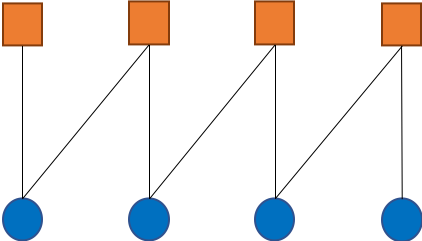
\includegraphics[scale=0.75]
	{pics/ira.png}
	\caption{Sebuah Tanner \textit{graph} untuk \textit{accumulator} dengan $\mathbf{H}$ pada (\ref{eq: IRA}).}
	\label{fig:ira codes}
\end{figure}
Dalam proses pengkodean, \textit{Low Density Generator Matrix} (LDGM) menggunakan operasi XOR. LDGM dapat di-\textit{decode} dengan \textit{Sum Product Algorithm} (SPA). Keuntungan dari pengkodean LDGM adalah proses yang sederhana \cite{LDGM}, karena hanya terdiri dari perkalian matriks dari input simbol dengan matriks \textit{sparse} generator $\mathbf{G}$. Matriks \textit{parity check} $\mathbf{H}$ LDGM \textit{codes} memiliki \textit{degree} satu dengan matriks identitas di dalamnya yang menunjukkan bahwa matriks tersebut sederhana dalam proses pembuatan matriks generator seperti matriks berikut
\begin{eqnarray}
\mathbf{H}=\begin{bmatrix}
0 & 1 & 0 & 0 & 1 & 0 & 0\\
1 & 0 & 1 & 0 & 0 & 1 & 0\\
1 & 0 & 0 & 1 & 0 & 0 & 1
\end{bmatrix}, \;
\mathbf{G}=\begin{bmatrix}
1 & 0 & 0 & 0 & 0 & 1 & 1\\
0 & 1 & 0 & 0 & 1 & 0 & 0\\
0 & 0 & 1 & 0 & 0 & 1 & 0\\
0 & 0 & 0 & 1 & 0 & 0 & 1
\end{bmatrix}.
\end{eqnarray}
LDGM \textit{codes} dikombinasikan dengan LDPC \textit{codes} sebagai \textit{parity} yang berfungsi untuk menjadi \textit{redundancy} dengan memberikan tambahan bit \textit{parity} pada \textit{codeword} $\mathbf{c}$. Parameter $\mathbf{c}$ merupakan bit informasi $\mathbf{b}$ yang telah diberi bit \textit{parity} untuk menambah kemampuan dalam koreksi kesalahan. 

\section{Algoritma \textit{Progressive Edge-Growth} (PEG)}

\textit{Progressive Edge-Growth} (PEG) adalah salah satu metode dalam merancang matriks \textit{parity check} LDPC \textit{codes} berdasarkan dari Tanner \textit{graph} dengan memperhatikan penyebaran \textit{edge} yang terhubung pada setiap \textit{node} untuk menghasilkan \textit{girth} besar \cite{PEG}. Perancangan LDPC \textit{codes} dengan menggunakan PEG dapat dibuat berdasarkan jumlah \textit{variable nodes} atau \textit{block length} $n$, check node $m$, VND, dan CND. PEG melakukan penyebaran \textit{edge} menggunakan graf pohon dengan memperhatikan \textit{degree} setiap \textit{node} yang telah ditentukan dan setiap \textit{node} hanya muncul sekali saja. Kedalaman dari graf pohon akan disimbolkan dengan $l$.

Secara sederhana proses pembuatan LDPC \textit{codes} menggunakan algoritma PEG adalah sebagai  berikut \cite{PEG}:
\begin{enumerate}
	\item Tempatkan elemen 1 mulai dari kolom ke-1 sampai ke-$n$, penempatan ini memperhatikan baris atau \textit{check node} dengan \textit{degree} terkecil.
	\item Menyebarkan \textit{edge} ke \textit{node} yang belum terhubung dengan memperhatikan \textit{degree} dari \textit{check node}.
\end{enumerate}
\textit{Cycle} dari LDPC \textit{codes} yang terbentuk menggunakan PEG dapat dipastikan akan bernilai $2(l+2)$.
%\begin{equation}
%2(l+2).
%\end{equation}
Dalam perancangan LDPC \textit{codes} menggunakan algoritma PEG dengan nilai $d_v$, $d_c$, dan $m$ yang telah ditentukan, dapat diketahui batas dari nilai \textit{girth} melalui persamaan
\begin{equation}
t=\frac{\log\left ( md_c^{max}- \frac{md_c^{max}}{d_v^{max}} - m +1 \right )}{\log\left [ \left ( d_v^{max} -1  \right ) \left ( d_c^{max} -1  \right ) \right ]}-1
\label{eq:t}
\end{equation}
\begin{equation}
g \geq 2 \left (\left \lfloor t \right \rfloor +2 \right ),
\label{eq:g}
\end{equation}
dengan $g$ adalah \textit{girth}, dari Persamaan (\ref{eq:t}) dan (\ref{eq:g}) maka
\begin{equation}
\frac{d_v^{max}\left [  \left ( d_v^{max}-1 \right )^{t+1} \left ( d_c^{max}-1 \right )^{t+1} -1\right ]}{\left ( d_v^{max}-1 \right ) \left ( d_c^{max}-1 \right )-1}<m.
\end{equation}

PEG memiliki dua metode dalam proses perancangan LDPC \textit{codes} dengan cara \cite{PEG2}:
\begin{enumerate}
	\item Secara acak memilih \textit{check nodes} terkecil yang ditemukan.
	\item Selalu memilih \textit{check nodes} terkecil yang ditemukan sesuai dengan urutannya $c_1, c_2, c_3, \cdots, c_{m},$ $m$ adalah jumlah baris.
\end{enumerate}
Hal ini mengakibatkan LDPC \textit{codes} akan memiliki matriks \textit{parity check} berbeda, apabila menggunakan algoritma PEG.


\section{Modulasi}
Modulasi merupakan proses perubahan sebuah gelombang periodik menjadi sebuah sinyal yang mampu membawa informasi. Sinyal informasi akan ditumpangkan pada gelombang radio yang bertugas sebagai sinyal pembawanya (\textit{carrier}). Langkah terbaik untuk mengirimkan informasi yang berupa $+1$ atau $-1$ menggunakan gelombang radio dengan memodulasi sinyal \textit{carrier} dengan frekuensi $f_c$ yang sesuai sinyal informasinya \cite{modul}. Bentuk gelombang dari sinyal \textit{carrier} $S(t)$ dapat dinyatakan sebagai 
\begin{equation}
	S(t) =A \; cos \left \{ 2\pi f_c t + \theta \left( t \right ) \right \}
\end{equation}
dengan A adalah amplitudo, $f_c$ adalah frekuensi tengah, dan $\theta (t)$ adalah fasa sesuai dengan variansi waktu dari gelombang sinyal \textit{carrier}. 



\section{Pemodelan Kanal}
%-----------------------------------------------------------------------------%
Tugas Akhir ini menggunakan pemodelan kanal radio. Terdapat dua paramater utama dalam pemodelan kanal yang dirancang, yaitu adanya \textit{noise} dan terjadinya \textit{multipath fading}. Sub bab ini akan menjelaskan kanal AWGN dan \textit{frequency selective fading}.
%, \textit{Power Delay Profile} (PDP), dan pemodelan kanal Indonesia. 
\subsection{Kanal \textit{Additive White Gaussian Noise} (AWGN)}
\begin{figure}[tp]
	\centering
	
\includegraphics[scale=0.55]
		{pics/awgn1.png}
		\caption{Diagram blok kanal AWGN.}
	\label{fig:Model Channel Model AWGN}
\end{figure}
Kanal AWGN adalah kanal paling populer karena dianggap sebagai model yang baik untuk banyak aplikasi. Kanal AWGN memiliki beberapa karakteristik, antara lain \cite{awgn1}: 
\begin{enumerate}
\item \textit{Additive}, karena \textit{noise} ditambahkan ke simbol-simbolnya.
\item \textit{White}, memiliki rapat daya yang konstan di setiap frekuensi.
\item \textit{Gaussian}, karena \textit{noise} dari kanal AWGN terdistribusi \textit{Gaussian}.
\end{enumerate}
Pemodelan matematika untuk sinyal yang diterima di \textit{receiver} pada kanal AWGN berdasarkan Gambar \ref{fig:Model Channel Model AWGN} adalah 
\begin{equation}
r(t)=s(t)+n(t)
\label{eq:Model Matematika Channel Model AWGN}
\end{equation}
dengan $s(t)$ adalah sinyal yang ditransmisikan, $n(t)$ adalah \textit{white Gaussian noise}, dan $r(t)$ adalah sinyal yang diterima.

Proses transmisi pada kanal AWGN akan disimulasikan dengan menggunakan aplikasi MATLAB. Densitas spektral daya kanal AWGN sama rata untuk semua frekuensi. 
%Sumber \textit{noise} pada kanal AWGN berupa \textit{noise thermal} yang diakibatkan oleh kondisi panas komponen elektronik di \textit{receiver}.
Sinyal yang \text{diterima} dalam aplikasi MATLAB didefinisikan sebagai 
\begin{equation}
\mathbf{r}_{x}=\mathbf{H}\cdot \mathbf{t}_{x}+\mathbf{n}
\label{eq:AWGN matlab}
\end{equation}
dengan $\mathbf{r}_{x}$ merupakan sinyal yang diterima oleh \textit{receiver}, $\mathbf{h}=1$ untuk AWGN \textit{channel}. Parameter $\mathbf{t}_{x}$ adalah sinyal yang dikirimkan dari \textit{transmitter}, dan \textit{noise} $\mathbf{n}$ didefinisikan dengan perintah MATLAB
\begin{equation}
\mathbf{n}=\sigma \cdot (randn(1,B)) + \sqrt{-1} \times (randn(1,B)),
\end{equation}
yang memiliki distribusi Gaussian sepanjang simbol ($B$) dengan varians $\sigma^2$ pada (\textit{double-sided noise}) dan rata-rata nol. Probabilitas fungsi densitasnya adalah
\begin{equation}
p(m)=\frac{1}{\sigma \sqrt{2\pi}}\cdot \exp \left ( -\frac{m^2}{2\sigma ^{2}} \right )
\label{eq:prob dens}
\end{equation}
dengan $m$ adalah \textit{random} variabel dari \textit{noise}.
%$n(t)$ adalah contoh fungsi proses AWGN yang menggunakan proses \textit{probability density function} (pdf) dan rapat daya spektral 
%\begin{equation}
%\Phi_{nn}(f)=\frac{1}{2}N_{0}[W/Hz],
%\label{eq:Noise Channel Model AWGN}
%\end{equation}
%\noindent dengan $N_{0}$ bersifat konstan. AWGN \textit{Channel} memiliki model seperti pada Gambar \ref{fig:Model Channel Model AWGN}.  
\subsection{\textit{Frequency Selective Fading Channel}}
\begin{figure}[tb]
	\centering
	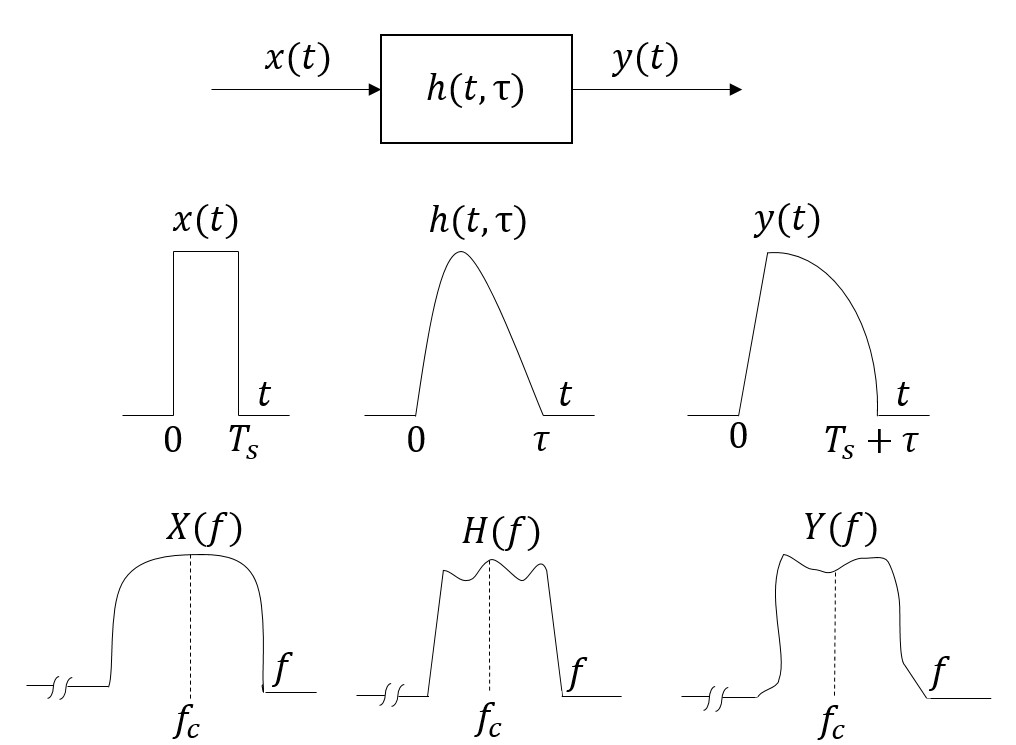
\includegraphics[scale=0.7]
	{pics/fadi.jpg}
	\caption{Karakteristik kanal untuk \textit{frequency selective fading}.}
	\label{fig:Frequency Selective Fading Channel}
\end{figure}
\textit{Frequency selective fading channel} terjadi ketika amplitudo konstan dan respon fasa linier pada \textit{wireless channel} lebih sempit daripada \textit{bandwidth} sinyal, sehingga amplitudo respon frekuensi dari sinyal yang ditransmisikan menjadi bervariasi terhadap frekuensi \cite{fading1}. Gambar \ref{fig:Frequency Selective Fading Channel} menunjukkan karakteristik dari \textit{frequency selective fading channel} dan ilustrasi di \textit{domain} waktu dan frekuensi. 
\textit{Frequency selective fading channel} adalah sebuah \textit{wideband channel} dengan kondisi kanal ($\tau$) lebih besar dari pada periode simbol sinyal yang ditransmisikan ($T_{s}$) atau jika \textit{maximum excess delay} ($T_{m}$) lebih besar daripada ($T_{s}$) \cite{fading2}. Sehingga dapat disimpulkan sinyal dipengaruhi oleh \textit{frequency selective fading channel} jika:
\begin{eqnarray}
B_{s} \geq B_{c},  \nonumber \\ 
 T_{s} \leq \sigma_{\tau}, \nonumber \\ 
T_{s} \leq T_{m}. 
\label{eq:Kondisi Frequency Selective Fading Channel}
\end{eqnarray}
\noindent Oleh karena itu, sebuah kanal dianggap \textit{frequency selective fading channel} ketika $\sigma_{\tau} = 0.1 T_{s}$.

%\section{Kanal \textit{Broadband}}
%Kanal \textit{broadband} identik dengan kanal yang memiliki \textit{bandwidth} transmisi yang lebih besar dari \textit{bandwidth} koheren dalam kanalnya. Kanal \textit{broadband} dibutuhkan oleh aplikasi-aplikasi dengan kecepatan pengiriman data yang tinggi, sebab kanal \textit{broadband} memiliki kapasitas yang sangat besar. \textit{Bandwidth} yang lebar menyebabkan kanal \textit{broadband} rentan terhadap efek kanal \textit{multipath fading} \cite{broadband}. Hal ini berkaitan dengan \textit{bandwidth} koheren yang lebih kecil daripada \textit{bandwidth} sinyal sehingga kanal akan mengalami \textit{frequency selective-fading}. Oleh sebab itu, OFDM atau \textit{equalizer} diperlukan untuk memproses sinyal yang diterima pada sisi penerima setelah melalui kanal \textit{broadband} sehingga \textit{diversity} dapat dicapai.

\section{\textit{Power Delay Profile} (PDP)}
\begin{figure}[b!]
	\centering
	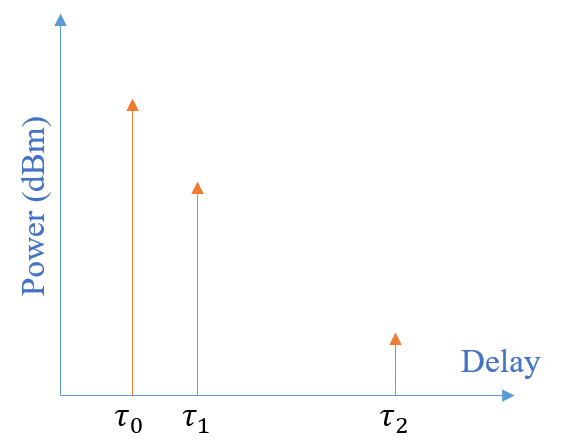
\includegraphics[scale=0.85]
		{pics/PDP.png}
		\caption{PDP pada \textit{multipath fading channel}.}
	\label{fig:PDP}
\end{figure}
\textit{Power Delay Profile} (PDP) merepresentasikan daya rata-rata sebagai fungsi \textit{delay} propagasi akibat \textit{multipath delay} yang dialami kanal. Daya yang diterima dan dispersifitas \textit{multipath} dalam saluran nirkabel dapat diprediksi berdasarkan nilai PDP. Kanal dapa mengalami \textit{multipath} akibat adanya refleksi (\textit{reflection}), pembiasan (\textit{refraction}), hamburan (\textit{scattering}), dan penyaluran (\textit{ducting}) sehingga menyebabkan interferensi \cite{pdp2}. Kanal \textit{multipath} menyebabkan adanya \textit{Inter-Symbol Interference} (ISI) yang dihasilkan dari pengaruh lingkungan jalur rambat antara pemancar dan penerima \cite{pdp1}. 

Dalam proses mengeplot PDP, sumbu $X$ mewakili \textit{delay} propagasi masing-masing \textit{path} dan sumbu $Y$ mewakili daya sinyal dari setiap \textit{path}. Gambar \ref{fig:PDP} menunjukkan contoh bagaimana sinyal yang ditransmisikan akan diterima pada sisi penerima dengan daya yang berbeda-beda melalui kanal \textit{multipath} berdasarkan \textit{delay} propagasi yang berbeda pula. PDP dicirikan dengan nilai \textit{maximum excess delay}, \textit{mean excess delay}, dan \textit{root mean square} (RMS) \textit{delay spread}.
%
%PDP atau \textit{multipath intensity profile} ($A_{c}(\tau)$) adalah daya di \textit{receiver} yang telah dipengaruhi oleh \textit{delay} dan perubahan fasa akibat dari \textit{multipath channel} \cite{pdp1}. \textit{Multipath channel} menyebabkan adanya \textit{Inter-Symbol Interference} (ISI) yang dihasilkan dari pengaruh lingkungan jalur rambat antara pemancar dan penerima. PDP digambarkan dalam grafik daya sinyal untuk setiap \textit{multipath} tergantung dari setiap \textit{propagation delays}-nya. Gambar \ref{fig:PDP} menunjukkan daya sinyal yang diterima di \textit{receiver} memiliki nilai berbeda dalam sebuah \textit{multipath channel} dengan propagation delays ($\tau_{0}, \tau_{1}, \tau_{2}$).     
%\begin{equation}
%p(\tau) = \int_{-\infty }^{\infty } S(f,\tau) df,
%\label{pdp}
%\end{equation}
 	
%\subsection{Pemodelan Kanal Indonesia}
%Model kanal Indonesia didapatkan melalui pengujian kondisi parameter lingkungan Indonesia. Untuk studi awal, representasi dari Indonesia menggunakan parameter lingkungan dari Kota Bandung \cite{ch1}. Keakuratan kanal model Indonesia bisa ditingkatkan dengan menambah sampel dari berbagai kota di Indonesia. Parameter lingkungan seperti tekanan udara, kelembapan, dan suhu yang didapat dari Badan Meteorologi Klimatologi, dan Geofisika (BMKG). Pemodelan kanal dapat menggunakan \textit{software} \textit{New York University Wireless Simulator} (NYUSIM) \text{dengan} parameter dari data rata-rata harian sehingga diharapkan dapat menghasilkan model kanal yang akurat. Kanal model di Kota Bandung dapat direpresentasikan sebagai \textit{multipath fading channel} yang memiliki 18~\textit{paths} dengan \textit{delay interval} 10~ns dan \textit{outage performance} Kota Bandung yang telah \text{divalidasi} secara teori. Hasil dari pemodelan kanal Indonesia yang terkhusus di Kota Bandung telah dibuktikan akan memiliki kinerja yang lebih baik dengan menggunakan \textit{channel coding} LDPC \textit{codes} atau Polar \textit{codes} \cite{ch1}.  



\begin{figure}[tb]
	\centering
	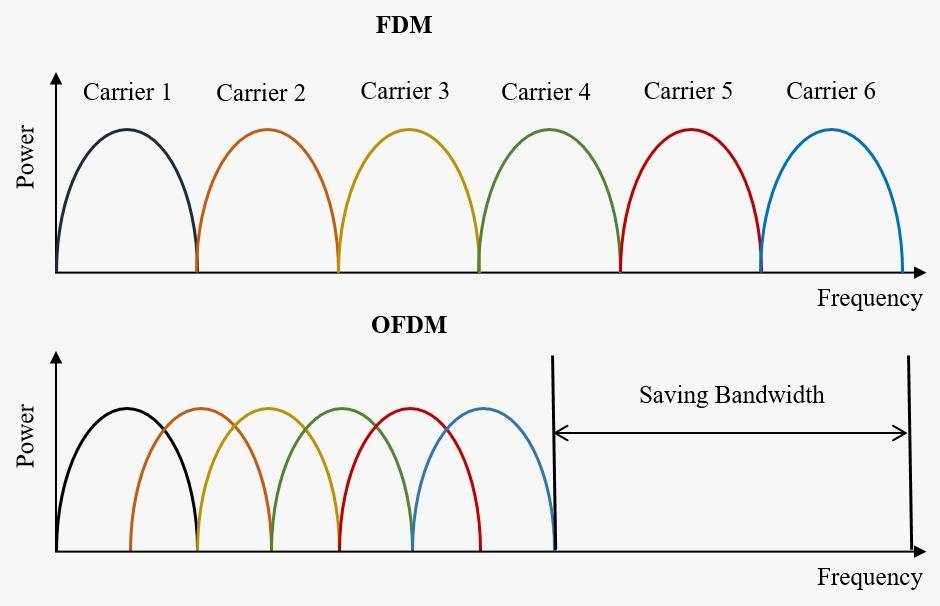
\includegraphics[width=1\textwidth]
	{pics/ofdm}
	\caption{Efisiensi spektrum dengan \textit{saving bandwidth} sebaga hasil OFDM dibandingkan dengan FDM.}
	\label{fig:OFDM}
\end{figure}
\section{\textit{Orthogonal Frequency Division Multiplexing} (OFDM) }
OFDM adalah sebuah skema untuk mengirimkan banyak informasi melalui satu saluran atau \textit{multicarrier modulation} dengan alokasi frekuensi tertentu yang sederhana dan sesuai untuk transmisi data berkecepatan tinggi melalui kanal \textit{multipath fading}. OFDM mampu mengubah kanal \textit{frequency-selective fading} menjadi kanal \textit{frequency-flat fading} dalam sistem transmisi paralel melalui kanal \textit{narrowband} \cite{ofdm}. OFDM mampu menghilangkan gangguan ISI dan \textit{Inter-Carrier Interference} (ICI) melalui penggunaan \textit{cyclic prefix} (CP). OFDM dianggap sebagai penerus teknik \textit{Frequency Division Multiplexing} (FDM) dengan cara menghilangkan ketidakefisienan dalam saluran seperti yang ditunjukkan oleh Gambar \ref{fig:OFDM} dengan memanfaatkan \textit{subcarriers} yang saling tegak lurus (\textit{orthogonal subcarriers}) \cite{ofdm2}.

\begin{figure}[tb]
	\centering
	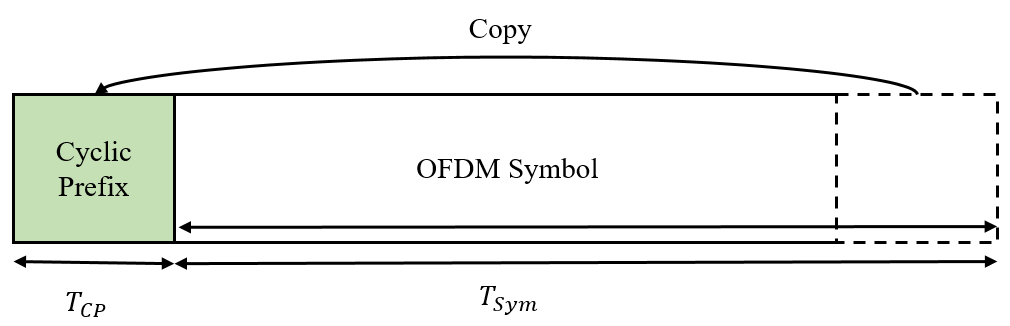
\includegraphics[width=1\textwidth]
	{pics/cyclicprefix}
	\caption{Ilustrasi penambahan CPpada awal OFDM simbol sebesar $T_{CP}$.}
	\label{fig:CP}
\end{figure}


\subsection{\textit{Cyclic Prefix} (CP)}
CP adalah awalan simbol OFDM yang merupakan pengulangan bagian akhir dari simbol OFDM seperti ditunjukkan pada Gambar \ref{fig:CP} dengan $T_{CP}$ adalah panjang CP dan panjang simbol informasi dinyatakan dengan $N$. CP digunakan dalam OFDM untuk mengatasi efek dari ISI akibat kanal \textit{multipath fading}. Simbol yang telah dilengkapi dengan CP akan mampu melakukan \textit{recovery} dengan baik pada sisi penerima walaupun terkena interferensi \textit{fading} dari kanal yang cukup besar. Dalam CP-OFDM, satu blok simbol kompleks dipetakan ke dalam satu pasang \textit{orthogonal carriers}. Arsitektur CP-OFDM memiliki kompleksitas yang rendah, karena penggunaan \textit{Inverse Fast Fourier Transform} (IFFT) dalam OFDM \cite{CP1}. Selain itu, panjang CP diusahakan sama atau lebih besar dari jumlah \textit{path} dalam PDP untuk menjamin kinerja sistem yang terbebas gangguan ISI. Penggunaan CP-OFDM secara umum memiliki dua tujuan, antara lain:
\begin{enumerate}
	\item Pemberian \textit{guard interval} untuk menghilangkan ISI yang disebabkan simbol sebelumnya.
	\item Penyalinan bagian akhir dari simbol yang menyebabkan konvolusi linier dari kanal \textit{frequency-selective fading} dapat dihitung sebagai konvolusi melingkar, sehingga mampu menyederhanakan proses estimasi kanal.
\end{enumerate}

\subsection{\textit{Inverse Fast Fourier Transform} (IFFT) }
IFFT adalah proses untuk menghasilkan simbol-simbol OFDM pada sisi pengirim dengan frekuensi daripada setiap informasinya akan dibuat saling tegak lurus (orthogonal). IFFT mengubah sebuah spektrum, yaitu amplitudo dan fasa dari setiap sinyal informasi ke bentuk sinyal dalam domain waktu \cite{fft}. IFFT mengubah sejumlah simbol bernilai kompleks ke dalam domain waktu dengan jumlah simbol yang tetap. \textit{Subcarrier} yang \textit{orthogonal} pada IFFT digunakan dalam sinyal OFDM agar dapat mengatur amplitudo dan fasa dari setiap simbol dengan mudah.

\subsection{\textit{Fast Fourier Transform} (FFT)}
FFT adalah proses pemisahan antara frekuensi \textit{carrier} dengan simbol OFDM yang diterima pada sisi penerima sebelum didemodulasi dan diubah kembali ke dalam bentuk bit. FFT juga digunakan untuk implementasi \textit{discrete fourier transform} agar lebih cepat dan efisien. Ukuran FFT (FFT \textit{size}) mengacu pada jumlah \textit{subcarrier} dari simbol OFDM yang diharapkan sesuai ukuran $2^N$, dengan $N$ adalah jumlah sampel yang diubah waktu ke domain frekuensi \cite{fft}. Oleh karena itu, ukuran FFT akan mempengaruhi jumlah simbol OFDM untuk setiap blok atau frame dari suatu sistem OFDM. Ukuran FFT ditentukan dengan memperhatikan keseimbangan antara perlindungan terhadap efek \textit{multipath}, pergeseran Doppler (\textit{Doppler shift}), dan kompleksitas sistem. Ukuran FFT yang semakin besar akan mengurangi \textit{subcarrier spacing} dan menambahkan durasi simbol. Hal ini akan memudahkan dalam melindungi simbol OFDM dari interferensi akibat \textit{multipath}. Di sisi lain, berkurangnya \textit{subcarrier spacing} akan membuat sistem lebih terhadap ICI akibat efek Doppler \textit{spread} dalam sistem komunikasi \textit{wireless}. 



\subsection{Matriks \textit{Circulant} dan Matriks \textit{Toeplitz}}
Matriks \textit{circulant} $\mathbf{H}_c$ adalah sebuah matriks \textit{Toeplitz} yang memiliki dimensi mengikuti jumlah CP dan FFT \textit{size}, jumlah baris $\mathbf{H}_c$ dinyatakan oleh
\begin{equation}
	m_{\mathbf{H}_c}=(F+Q \times 2)-1
\end{equation}
dengan $m_{\mathbf{H}_c}$ adalah baris dari $\mathbf{H}_c$, $F$ adalah FFT \textit{size}, dan $Q$ adalah panjang CP. Untuk kolom dari $\mathbf{H}_c$ dinyatakan oleh
\begin{equation}
	n_{\mathbf{H}_c}=F+Q.
\end{equation}

Sifat dari matriks \textit{circulant} yang mudah diturunkan membuat matriks ini dapat digunakan untuk memperkirakan dan menjelaskan perilaku dari matriks \textit{Toeplitz} dengan baik, salah satunya seperti yang terjadi dalam sinyal terima di \textit{receiver} $\mathbf{y}$ yang dinyatakan menurut 
\begin{equation}
\mathbf{y}= \mathbf{H}_c \cdot \mathbf{x}+ \mathbf{n},
\label{matrixeq}
\end{equation} 
dengan $\mathbf{H}_c$ adalah matriks \textit{circulant} yang berisi nilai \textit{path} yang merepresentasikan kondisi kanal. Apabila sebuah kanal memiliki \textit{path} $\mathbf{h}=[~1 ~0.9 ~0.8]$ dan bit yang dikirimkan $\mathbf{x}$ ditambah dengan CP menjadi $\mathbf{x}_{cp}=[c d: a b c d]$, maka sinyal yang diterima dinyatakan menjadi
\begin{equation}
\textbf{y} = \begin{bmatrix}
1   & 0   & 0   & 0   & 0   & 0\\ 
0.9 & 1   & 0   & 0   & 0   & 0\\ 
0.8 & 0.9 & 1   & 0   & 0   & 0\\ 
0   & 0.8 & 0.9 & 1   & 0   & 0\\ 
0   & 0   & 0.8 & 0.9 & 1   & 0\\ 
0   & 0   & 0   & 0.8 & 0.9 & 1\\ 
0   & 0   & 0   &  0  & 0.8 & 0.9\\ 
0   & 0   & 0   &  0  & 0   & 0.8
\end{bmatrix}
\begin{bmatrix}
c\\ 
d\\ 
a\\ 
b\\ 
c\\ 
d
\end{bmatrix}
+ \begin{bmatrix}
n_{1}\\ 
n_{2}\\ 
n_{3}\\ 
n_{4}\\ 
n_{5}\\ 
n_{6}\\ 
n_{7}\\ 
n_{8}
\end{bmatrix}~,\\
\end{equation}



%\begin{equation}
%H=\begin{bmatrix}  
%\tikzmarknode{m1}{c}\\ 
%\tikzmarknode{m3}{0.9c + d} \\ 
%0.8c + 0.9d + a \\ 
%0.8d + 0.9a + b\\ 
%0.8a + 0.9b + c \\ 
%0.8b + 0.9c + d\\ 
%\tikzmarknode{m2}{0.8c + 0.9d}\\ 
%\tikzmarknode{m4}{0.8d}
%\end{bmatrix}
%\end{equation}




\begin{equation}
\mathbf{y} = \begin{bmatrix}
\tikzmarknode{m1}{c}\\ 
\tikzmarknode{m3}{0.9c + d} \\ 
0.8c + 0.9d + a \\ 
0.8d + 0.9a + b\\ 
0.8a + 0.9b + c \\ 
0.8b + 0.9c + d\\ 
\tikzmarknode{m2}{0.8c + 0.9d}\\ 
\tikzmarknode{m4}{0.8d}
\end{bmatrix}
+ \begin{bmatrix}
\tikzmarknode{n1}{n_{1}}\\ 
\tikzmarknode{n3}{n_{2}}\\ 
n_{3}\\ 
n_{4}\\ 
n_{5}\\ 
n_{6}\\ 
\tikzmarknode{n2}{n_{7}}\\ 
\tikzmarknode{n4}{n_{8}}
\end{bmatrix}~,
\end{equation}  
\AddToShipoutPictureBG{%
	\begin{tikzpicture}[overlay,remember picture]
	\node[fill=gray!70,rounded corners,fit=(m1)(m3)]{};
	\node[fill=gray!70,rounded corners,fit=(m2)(m4)]{};
	\node[fill=gray!70,rounded corners,fit=(n1)(n3)]{};
	\node[fill=gray!70,rounded corners,fit=(n2)(n4)]{};
	%	\node[fill=purple!60,inner xsep=1.6ex,rounded corners,fit=(m2)(m3)]{};
	\end{tikzpicture}
}
Setelah CP dihapus dengan menghapus bagian yang berwarna abu-abu, sinyal yang diterima menjadi 
\begin{equation}
\mathbf{y} = \begin{bmatrix} 
0.8c + 0.9d + a \\ 
0.8d + 0.9a + b\\ 
0.8a + 0.9b + c \\ 
0.8b + 0.9c + d\\ 
\end{bmatrix}
+ \begin{bmatrix}
n_{3}\\ 
n_{4}\\ 
n_{5}\\ 
n_{6}\\ 
\end{bmatrix}~, \\ 
\end{equation}
yang ekivalen dengan
\begin{eqnarray}
\mathbf{y} &=&  \begin{bmatrix}
1   & 0    & 0.8   & 0.9 \\ 
0.9 & 1   & 0   & 0.8    \\ 
0.8 & 0.9 & 1   & 0     \\ 
0   & 0.8 & 0.9 & 1     \\ 
\end{bmatrix}
\begin{bmatrix}
a\\ 
b\\ 
c\\ 
d 
\end{bmatrix}
+ \begin{bmatrix}
n_{1}\\ 
n_{2}\\ 
n_{3}\\ 
n_{4}
\end{bmatrix}~,\\
&=& \mathbf{H}_c\cdot \mathbf{x} + \mathbf{n}.
\end{eqnarray}


\section{\textit{Signal-to-Noise Power Ratio} (SNR)}
\textit{Signal-to-Noise Power Ratio} (SNR) adalah rasio antara amplitudo sinyal data yang diinginkan $P_{signal}$ dan amplitudo \textit{noise} $P_{noise}$ dalam kanal tranmisi pada waktu tertentu. SNR digunakan untuk mengukur kualitas sebuah kanal transmisi. Apabila SNR semakin tinggi, maka semakin mudah juga untuk mengidentifikasi dan mengisolasi sumber \textit{noise} pada kanal. SNR bernilai nol menunjukkan bahwa sinyal data hampir tidak dapat dibedakan dari \textit{noise} yang ada. Penurunan SNR juga berpengaruh pada penurunan \textit{throughput} yang disebabkan oleh kesalahan yang terjadi di beberapa paket data \cite{SNR}. SNR $\gamma$ biasanya dinyatakan secara logaritmik dalam desibel (dB) menurut
\begin{figure}[b!]
	\centering	
	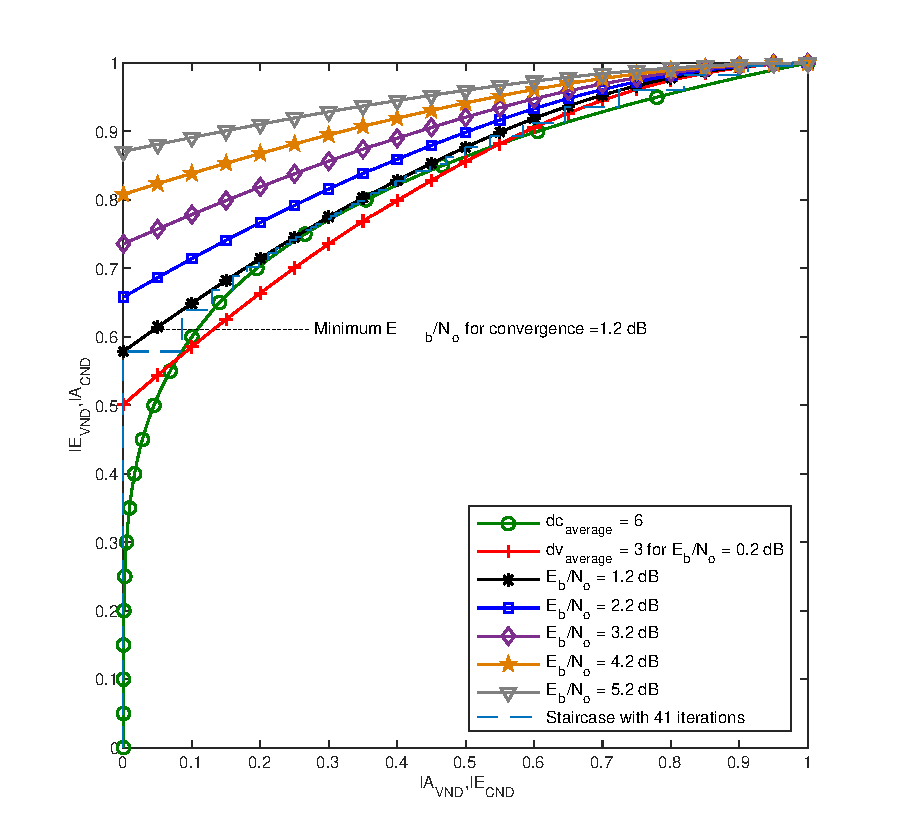
\includegraphics[width=1\textwidth]
	{pics/exit.pdf}
	\caption{EXIT \textit{chart} LDPC \textit{codes} untuk $d_{v}=3$ dan $d_{c}=6$ pada berbagai $E_b/N_0$.}
	\label{fig:EXIT chart}
\end{figure}
\begin{equation}
	\gamma = \frac{P_{signal}}{P_{noise}}.
\end{equation}

%-----------------------------------------------------------------------------%

\section{\textit{Extrinsic Information Transfer} (EXIT) \textit{Chart} }

EXIT \textit{chart} pertama diperkenalkan oleh Stephan ten Brink untuk menganalisis informasi timbal balik di \textit{decoder} dengan menggunakan proses \textit{iterative} dan untuk mengetahui jumlah iterasi yang diperlukan agar \textit{decoding} sukses \cite{exit23}. Proses dari transfer informasi direpresentasikan dalam bentuk grafik. Informasi yang masuk \textit{decoder} atau belum di-\textit{decode} disebut \textit{apriori mutual information} ($I_{A}$), sedangkan informasi yang keluar dari \textit{decoder} atau telah di-\textit{decode} disebut \textit{extrinsic mutual information} ($I_{E}$). EXIT \textit{chart} menganalisis menggunakan dua \textit{decoder} dan keluaran \textit{decoder} pertama adalah masukan \textit{decoder} kedua. Lalu di iterasi kedua, keluaran \textit{decoder} kedua menjadi masukan \textit{decoder} pertama dan begitu seterusnya. EXIT \textit{chart} direpresentasikan menggunakan grafik dengan mengeplot kinerja kedua \textit{decoder} dengan sumbu yang saling berlawanan. Kurva yang dihasilkan menggunakan fungsi \textit{staircase} yang dimulai dari titik ($0,0$) ketika tidak ada informasi timbal balik dan \textit{decoding} berhasil ketika mencapai titik ($1,1$) seperti pada Gambar \ref{fig:EXIT chart}. 		\ClearShipoutPicture

\begin{figure}[t!]

	\centering
	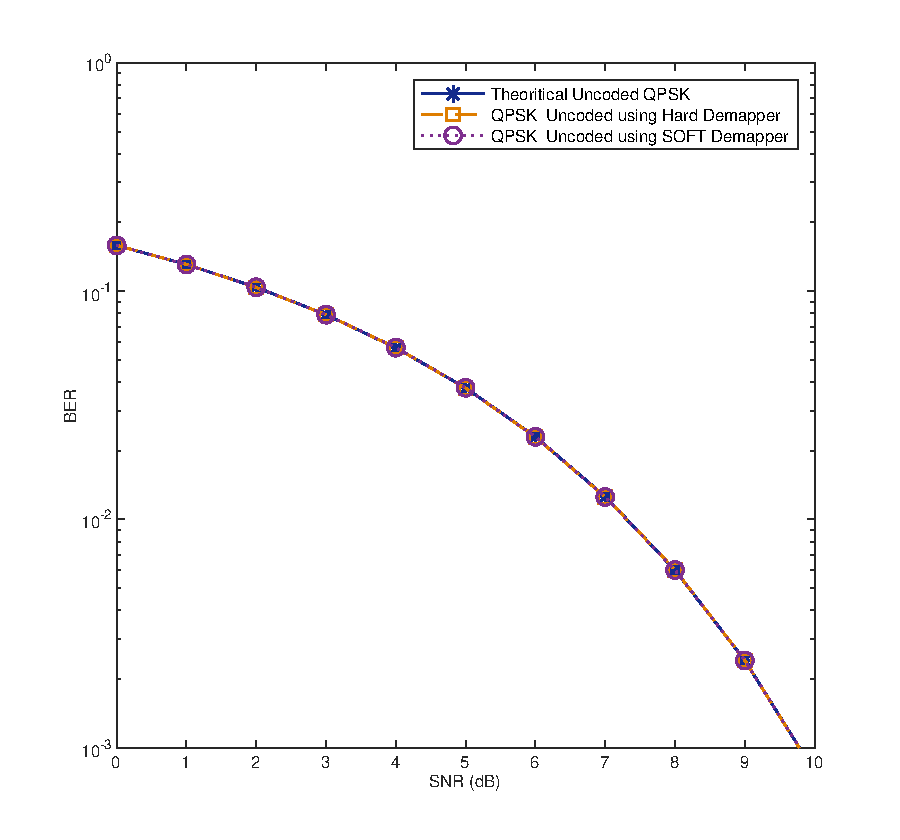
\includegraphics[width=1\textwidth]
	{pics/uncoded.pdf}
	\caption{Kinerja BER \textit{Uncoded} BER QPSK pada kanal AWGN dibandingkan dengan BER teori QPSK.}
	\label{fig:BER}

\end{figure}

\section{\textit{Bit Error Rate} (BER)}
Saat ini, segala komunikasi telah beralih ke bentuk komunikasi digital. Salah satu parameter pengukuran kinerja dari komunikasi digital menggunakan BER. Nilai BER didapat dari membandingkan bit yang diterima dengan bit yang ditransmisikan di sebuah sistem elektronika, antena, dan \textit{signal path} \cite{ber1}. Untuk di kanal AWGN, BER adalah kinerja yang dipengaruhi langsung oleh \textit{noise channel} dan untuk di \textit{fading channel} BER akan menjadi lebih buruk \cite{ber2}.
Persamaan sederhana BER adalah
\begin{equation}
BER=\frac{jumlah \; bit \; error}{total \; bit \; yang \; dikirimkan}.
\label{eq: Persamaan BER sederhana}
\end{equation} % From here on no logo
Perhitungan BER dalam teori tersebut untuk modulasi QPSK pada kanal AWGN dinyatakan oleh
\begin{equation}
BER_{QPSK\_AWGN}=\frac{1}{2} \mathrm{erfc} \left(  \sqrt{\frac{\gamma}{2} }  \right)
\end{equation}
dengan $\gamma$ adalah SNR. BER teori untuk modulasi QPSK pada kanal \textit{singlepath} dinyatakan dengan 
\begin{equation}
BER_{QPSK-Fading}= \frac{1}{2}\left [ 1-\frac{1}{\sqrt{1+\frac{2}{\gamma}}} \right ].
\end{equation} 

%\section{\textit{Bit Error Rate} (BER)}
%\begin{figure}[tb]
%\centering
%	\includegraphics[scale=0.52]
%		{pics/jadin.png}
%		\caption{Nilai \textit{Uncoded} BER QPSK pada AWGN \textit{channel}.}
%	\label{fig:BER}
%\end{figure}
%Saat ini, segala komunikasi telah beralih ke bentuk komunikasi digital. Salah satu parameter pengukuran kinerja dari komunikasi digital menggunakan BER. Nilai BER didapat dari membandingkan bit yang diterima dengan bit yang ditransmisikan di sebuah sistem elektronika, antena, dan \textit{signal path} \cite{ber1}. Untuk di  AWGN \textit{channel}, BER adalah kinerja yang dipengaruhi langsung oleh \textit{noise channel} dan untuk di \textit{fading channel} BER akan menjadi lebih buruk \cite{ber2}.
%Persamaan sederhana BER adalah
%\begin{equation}
%BER=\frac{jumlah \; bit \; error}{total \; bit \; yang \; dikirimkan}.
%\label{eq: Persamaan BER sederhana}
%\end{equation}
% 
%\textit{Noise} merupakan parameter yang mempengaruhi terjadinya BER, contoh penyebab terjadinya \textit{noise} adalah \textit{fading} dan pengaruh suhu alat. Pada AWGN \textit{channel}, \textit{noise} direpresentasikan dalam bentuk distribusi \textit{Gaussian}, sedangkan pada \textit{fading channel}, \textit{noise} direpresentasikan dalam distribusi \textit{Rayleigh} atau \textit{Ricean}. Berdasarkan dari fasa dan frekuensi pembawa, BER dapat didefinisikan sebagai berikut
%\begin{equation}
%P_{b}=\frac{2(1-\frac{1}{L})}{\log_{2}L}Q\left [ \sqrt{\left ( \frac{3\log_{2}L}{L^{2}-1} \right )} \frac{2E_{b}}{N_{o}} \right ],
%\label{eq: Rumus BER}
%\end{equation} 
%dengan nilai $L$ adalah jumlah \textit{level} di setiap dimensi dari \textit{M-ary} sistem modulasi, $E_{b}$ adalah energi setiap bit, dan $\frac{N_{0}}{2}$ adalah rapat daya \textit{noise}.


  
   
